\section{Introduction}

Statistical Model Checking techniques (SMC)\cite{Younes2004Planning,Sen2004Statistical,herault2004} can be seen as a trade-off between testing and formal verification. Recently, SMC has been an alternative to standard model-checking in order to avoid the state-space explosion problem, especially for verifying Cyber-physical Systems (CPSs) \cite{Yoo2016Challenges}. The core idea of SMC is to decide whether the stochastic model satisfies a given property or to evaluate its probability of satisfaction by combining statistical techniques with Monte-Carlo simulation on model traces. Nowadays, SMC is getting increasing industrial attention and there are many model checkers which support SMC techniques to analyze the stochastic model more effectively (e.g., Uppaal-SMC \cite{Bulychev2012UPPAAL}, Prism \cite{Kwiatkowska2002PRISM}).

CPS focus on the coupling of cyber part viewed as distributed computation units and physical part covering the environment affecting the running of the system. The modeling of stochastic behaviors for CPS might be highly cumbersome \cite{basu2010statistical} and the analysis of these models demands extremely high confidence \cite{du2015smc4rare}. SMC still encounters the performance bottleneck for verifying CPS. There are two factors having a direct influence on the performance of SMC, one is the huge number of simulation traces, the other is the length of a single trace. Both of them affect the performance of SMC. In this paper, we focus on these two factors to improve the efficiency of SMC. Figure \ref{tech-map} is the technology roadmap of our approach. A statistical model checker contains three components: simulator, SMC algorithm and model checker. The simulator generates simulation traces. Depending on the property
language, the checker verifies the traces and returns observations ( boolean or numerical values). The SMC algorithm collects observations obtained from a checker component and computes the probability. To reduce the number of simulation traces, we have proposed abstraction and learning teachique with SMC algorithm called AL-SMC \cite{jiangkaiqiang2016}. Through many experiments, we find that AL-SMC effectively reduces the number of traces, thereby improving the performance of SMC. As observed in \cite{younes2005ymer}, SMC can be distributed based on master/slave architecture where several slave computers are used to generate simulation traces. Inspired by it, we use distributed technology with simulator to reduce the time consumption for generating a single trace. Besides, we propose the distributed Bayesian Interval Estimation (BIE) algorithm \cite{zuliani2013bayesian}. In this paper, we combine distributed technology with AL-SMC technique, which is called DAL-SMC. The DAL-SMC technique reduces both the number of simulation traces and the time consumption for generating a single trace.

\begin{figure}[htbp]
	{
	\centering	
	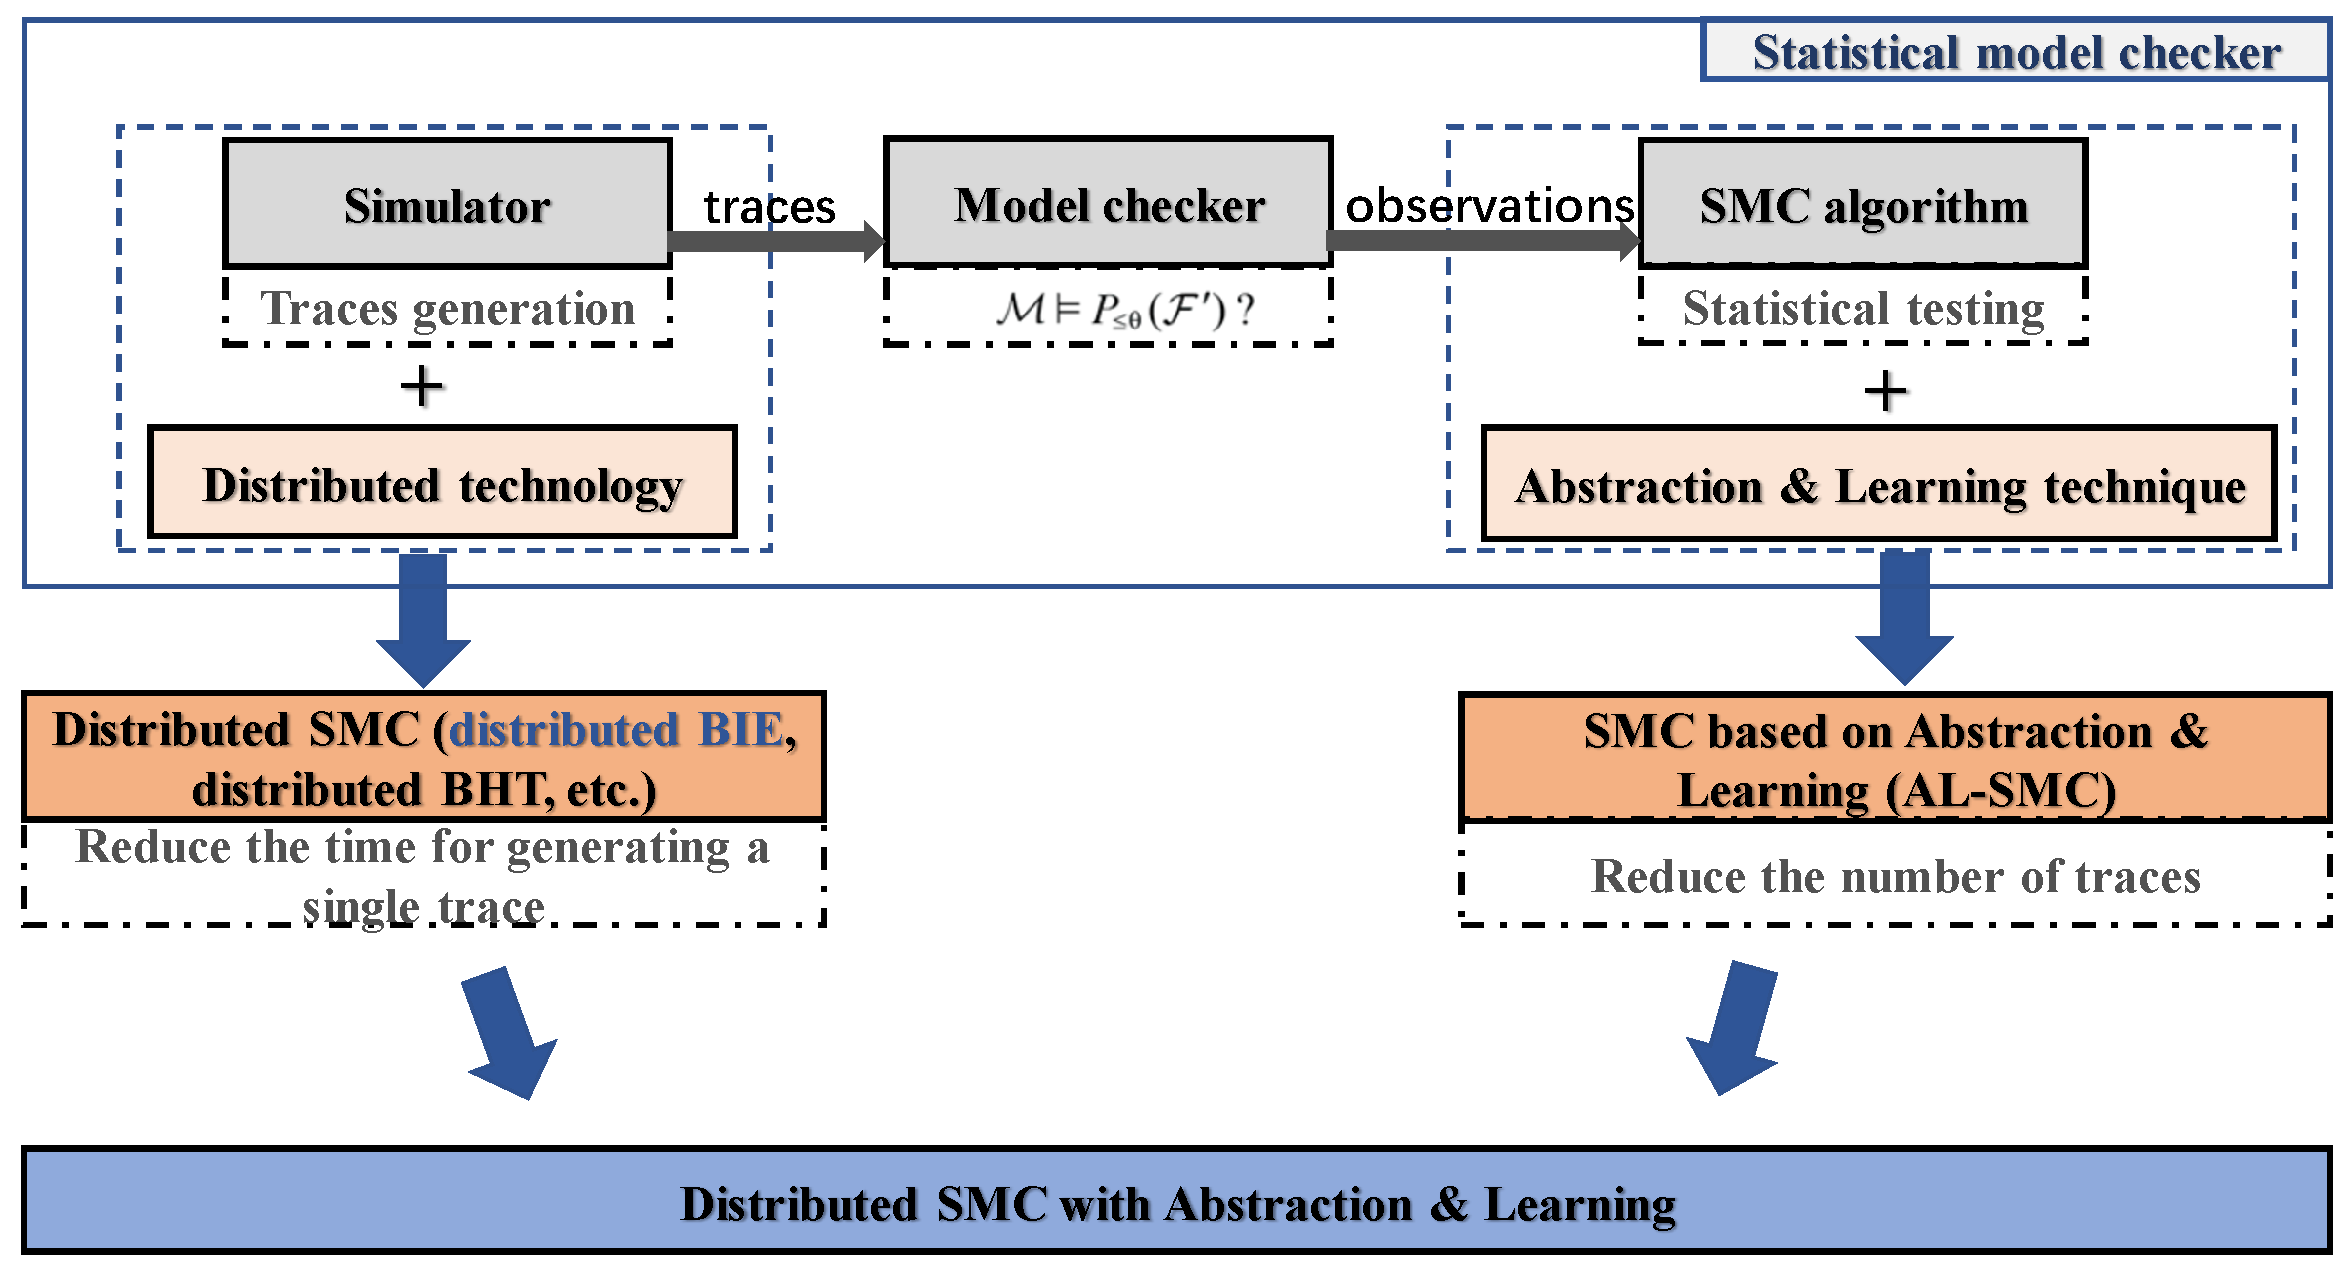
\includegraphics[width=3.0in,height=1.8in]{fig/paper-framework.png}
\caption{Technology roadmap.}\label{tech-map}	
	}
	%\vspace{0.10in}
	
\end{figure}

\textbf{The main contributions of this paper include:} (i)We propose a novel verification framework, which applies distributed technology to improve the efficiency of SMC. (ii)We propose the distributed BIE and DAL-SMC algorithms on the framework. The parameter optimization method is introduced to reduce the statistical error of DAL-SMC. This work is an extension of our previous work \cite{jiangkaiqiang2016}. (iii)The distributed BIE and DAL-SMC algorithms are implemented in our ModanaOnline platform  \cite{Cheng2015Modana} (https://github.com
/ECNU-MODANA/M
odana-Online) to support the automatic process. (iv)Sev
eral experiments are conducted to demonstrate that our approach effectively reduces the time consumption within an acceptable error bound.

The remainder of this paper is organized as follows. In Section 2, we present the framework of our approach, several core algorithms of distributed BIE and DAL-SMC in details. Parameter optimization method of DAL-SMC is also presented. Section 3 provides the algorithm analysis of DAL-SMC. Section 4 presents our implementation in ModanaOnline platform. Several experiments are conducted with three benchmarks. The experimental results show that our DAL-SMC are efficient and feasible. The related work is discussed in Section 5. Finally, conclusions and directions of future research are presented in Section 6. 